\documentclass[12pt,letterpaper]{article}
\usepackage[utf8]{inputenc}
\usepackage{amsmath}
\usepackage{amsfonts}
\usepackage{amssymb}
\usepackage{graphicx}
\usepackage[left=2cm,right=2cm,top=2cm,bottom=2cm]{geometry}

\usepackage{subfigure}

\author{Tanmoy Sanyal}
\title{CMPSC 240A HW-2 Report}

\begin{document}
\maketitle

\section*{Brief code summary}
\noindent I have worked only on the model problem for this assignment. The cgsolve iterations are built into main.c and the other relevant routines \texttt{daxpy()}, \texttt{ddot()} and \texttt{matvec()} are written separately. \texttt{genB} gives a preliminary wrapper for building the vector \textbf{b} from the harness function \texttt{cs240\_getB()}. Other modifications include: changing \texttt{save\_vec()} to output input parameters and output statistics in the header of \texttt{xApprox.txt}, and an option to verify the solution using the harness function \texttt{cs240\_verify()}. Note that this option requires assembling the global vector on the root processor and is hence turned off during the scaling experiments (set up by \texttt{scaling.py}).

\noindent The communication volume for 1 \texttt{matvec()} can be calculated as:
\begin{align*}
v & = 2(p-2) * BLOCK\_SIZE + 2 * BLOCK\_SIZE \\
  & = 2(p-1)*BLOCK\_SIZE
\end{align*}
\noindent, where $BLOCK\_SIZE = n/p$ is the size of the vector passed to each processor. I have also assumed a send and its corresponding receive as a single operation.

\section*{Solution verification}
\noindent The harness routine verifies my solution as correct only for small k values. Here is a graphical comparison (both cases calculated from my laptop).
%
\begin{figure*}[h]
\centering
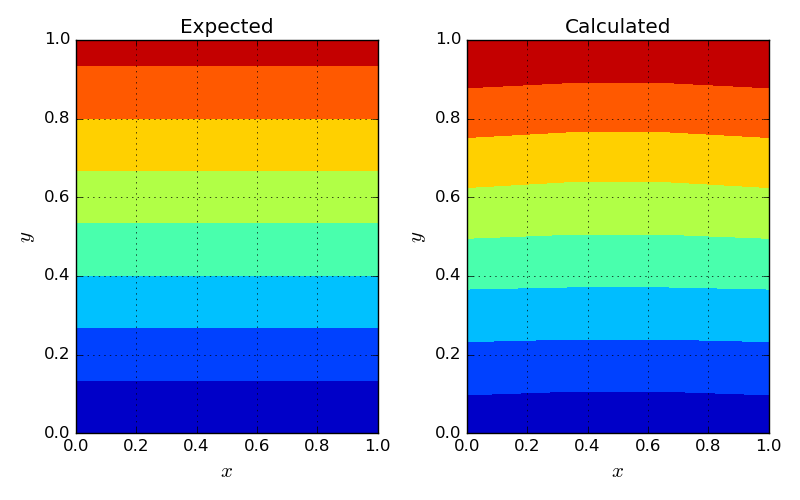
\includegraphics[scale = 0.45]{verify_k4.png}
\caption{$k = 4, p = 4$}
\end{figure*}
%
\begin{figure*}
\centering
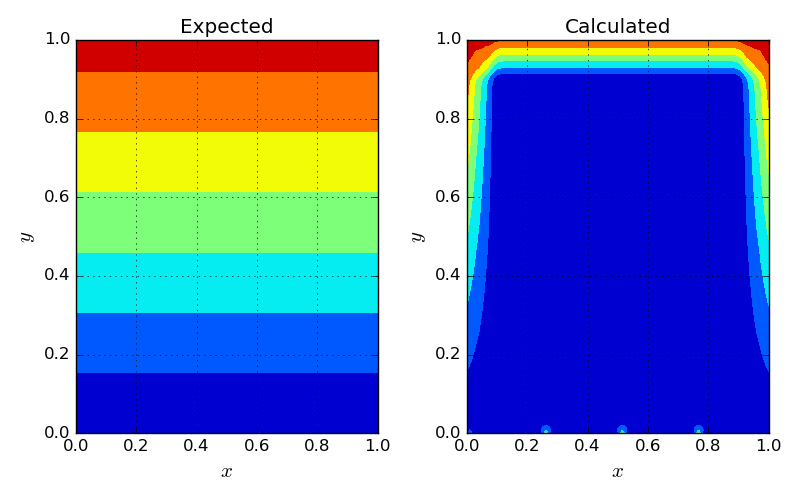
\includegraphics[scale = 0.45]{verify_k100.png}
\caption{$k = 100, p = 4$}
\end{figure*}

\section*{Scaling analyses}
\noindent The strong scaling experiment was run with $p = 1, 2, 4, 8, 12, 16, 24, 48, 72$ cores. Comet's compute nodes have cores that are multiples of 24, which guided this particular choice of higher $p$ values. $k = 64 * 24 = 1536$ on a single processor with 1000 CG iterations was found to take around 32 sec. With this value of k, the strong scaling looks like:
%
\begin{figure*}[h]
\centering
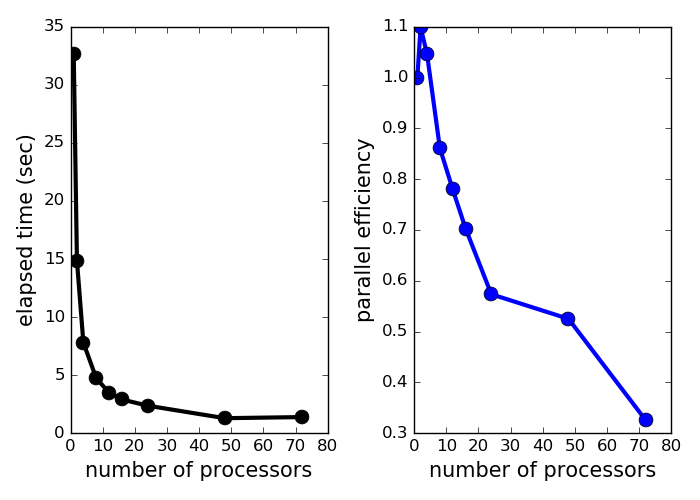
\includegraphics[scale = 0.7]{strongscale.png}
\caption{Strong scaling for $ k = 1536$}
\end{figure*}
%
\newpage
\noindent The weak scaling experiment used a similar number of processors as the previous case. However the first $k$ value was set at 144. This ensures that $k^2/p$ is always an integer and the tests run fast, even with 1000 iterations of the CG loop. Subsequent value of $k$ were chosen as $144 * int(sqrt(k))$. The weak scaling is:
%
\begin{figure*}[h]
\centering
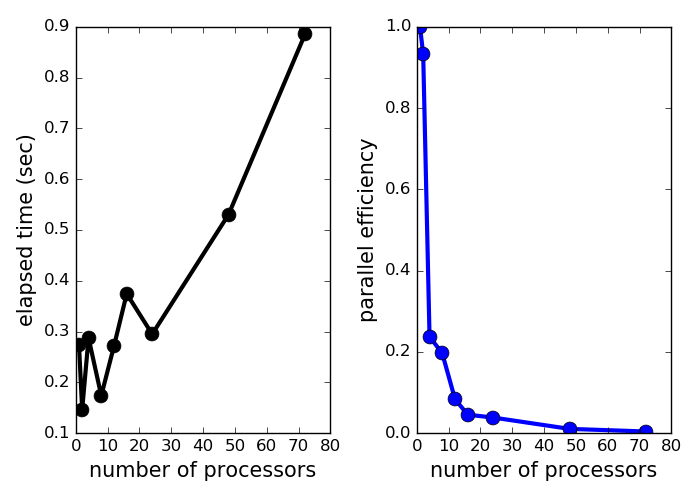
\includegraphics[scale = 0.7]{weakscale.png}
\caption{Weak scaling}
\end{figure*}

\end{document}